\documentclass[addpoints]{exam}

% \pagestyle{empty}                       %no page numbers
% \thispagestyle{empty}                   %removes first page number
% \setlength{\parindent}{0in}               %no paragraph indents

\usepackage{fullpage}
\usepackage[tmargin = 0.5in, bmargin = 1in, hmargin = 1in]{geometry}     %1-inch margins
\geometry{letterpaper}                  
\usepackage{graphicx}
\usepackage{amssymb}

% Default packages
\usepackage{latexsym}
\usepackage{amsfonts}
\usepackage{amsmath}
\usepackage{amsthm}
\usepackage{hyperref}
\usepackage{multicol}
\usepackage{multirow}
\usepackage{enumerate}
\usepackage{enumitem}


%% Definitions
\def\va{\mathbf{a}}
\def\vb{\mathbf{b}}
\def\vc{\mathbf{c}}
\def\vx{\mathbf{x}}
\def\vzero{\mathbf{0}}



\def\vi{\mathbf{i}}
\def\vj{\mathbf{j}}
\def\vk{\mathbf{k}}
\def\vr{\mathbf{r}}
\def\vu{\mathbf{u}}
\def\vv{\mathbf{v}}
\def\pageturn{\vfill
\begin{flushright}
	\begin{small}
		Continued $\rightarrow$
	\end{small}
\end{flushright}
\newpage}

\pagestyle{headandfoot}
\runningheadrule
\firstpageheader{\textbf{MTH 201-07 (Talbert)}}{\textbf{In-Class Assessment --- \numpoints \ points}}{\textbf{September 19, 2013}}
\runningheader{MTH 201}
{MTH 201-07 Assessment 1, Page \thepage\ of \numpages}
{Sept 19, 2013}
\firstpagefooter{}{}{}
\runningfooter{}{}{}

\begin{document}

		
\vspace*{0pt}

\noindent
Name: \underline{\hspace{2in}} \\


\noindent
\textbf{Instructions}:  You may use a $3 \times 5$ notecard with notes on it as well as a calculator. Except on multiple choice questions, you need to show all work in a clear and complete way to receive credit. The Assessment will end promptly at 12:50pm unless you have made alternate arrangements. 

\begin{questions}

\uplevel{\emph{Items 1---10 are multiple choice questions that address a variety of learning objectives. Please circle the ONE response you believe is most correct. You do not need to justify your answer.}}

\question[2] The derivative $f'(a)$ of a function $f$ at the point $x=a$ tells us
	\begin{parts}
		\part The average rate of change of $f$ at $x = a$
		\part The slope of the tangent line to $f$ at $x=a$
		\part The height of the graph of $f$ at $x = a$
		\part All of the above
		\part Just (a) and (b)
	\end{parts}

\question[2] A function $y = f(x)$ is such that the units of $x$ are in feet and the units of $y$ are in hours. The units of the derivative $f'(x)$ are 
	\begin{parts}
		\part Feet 
		\part Hours
		\part Feet per hour
		\part Hours per foot
		\part Feet per hour per hour
	\end{parts}
	
\question[2] For any function $y = g(x)$, if $g''(x) > 0$, it means that 
	\begin{parts}
		\part $g$ is positive 
		\part $g$ is increasing
		\part $g$ is linear with a positive slope
		\part $g$ is concave up
		\part No conclusions can be drawn about $g$ based on this information
	\end{parts}

\question[2] A function $y = g(x)$ is such that $g'(2) = -3$. From this information alone, we can conclude that 
		\begin{parts}
			\part The graph of $g$ is below the $x$-axis at $x = 2$
			\part The graph of $g$ is decreasing at $x = 2$
			\part The graph of $g$ is concave down at $x = 2$
			\part Just (a) and (b)
			\part None of the above
		\end{parts}

\question[2] A function $y = j(x)$ is such that $j(2) = 10$ and $j'(2) = -2$. The best  estimate to the value of $j(2.5)$ is 
			\begin{parts}
				\part 8
				\part 9
				\part 9.5
				\part 10.5
				\part 11
			\end{parts}
			
\pageturn

\question[2] Which of the following is a correct definition of the derivative of a function $f(x)$? 
\begin{parts}
	\part $\displaystyle{\lim_{h \to 0} \frac{f(x+h) - f(x)}{h}}$
	\part $\displaystyle{\lim_{x \to 0} \frac{f(x+h) - f(x)}{h}}$
	\part $\displaystyle{\lim_{h \to x} \frac{f(x+h) - f(x)}{h}}$
	\part $\displaystyle{\lim_{x \to h} \frac{f(x+h) - f(x)}{h}}$
	\part $\displaystyle{\lim_{h \to 0} \frac{f(h) - f(x)}{h}}$
\end{parts}

\question[2] Suppose a car is moving down a highway, and its position $s$ (in miles) from its starting point $t$ hours after it begins moving is given by a function $s(t)$. Suppose also that $s(2) = 75$ and $s'(2) = 80$. The best interpretation of these data is: 
	\begin{parts}
		\part After 2 hours, the car is 75 miles from its starting point and is traveling at 80 miles per hour. 
		\part After 2 hours, the car is 80 miles from its starting point and is traveling at 75 miles per hour. 
		\part After 2 hours, the car is traveling at 75 miles per hour and accelerating at a rate of 80 miles per hour per hour. 
		\part After 2 hours, the car is traveling at 80 miles per hour and accelerating at a rate of 75 miles per hour per hour. 
		\part None of the above are correct interpretations
	\end{parts}


\question[2] Under which of the following conditions will a function $y = f(x)$ be continuous at a point $x = a$? 
	\begin{parts}
		\part $f(a)$ is defined
		\part $\displaystyle{\lim_{x \to a} f(x)}$ exists
		\part Both (a) and (b) but no further conditions are necessary
		\part Both (a) and (b), and additionally we must have $\displaystyle{f(a) = \lim_{x \to a} f(x)}$
		\part None of the above
	\end{parts}
	
\question[2] If a function $y = f(x)$ \underline{fails} to be differentiable at $x= a$, we can conclude that 
	\begin{parts}
		\part $f(a)$ does not exist
		\part $\displaystyle{\lim_{x \to a} f(x)}$ does not exist
		\part $f$ is not continuous at $x=a$
		\part Both (b) and (c)
		\part None of the above 
	\end{parts}

\question[2] The tangent line to the graph of a function $g$ at $x = 1$ has equation $L(x) = 4x - 1$, and $g(1) = 3$. The best approximation to $g(1.5)$ given this information is 
	\begin{parts}
		\part $g(1.5) \approx 3.5$
		\part $g(1.5) \approx 5$ 
		\part $g(1.5) \approx 7$
		\part $g(1.5) \approx 9$
		\part Not enough information
	\end{parts}


\pageturn

\uplevel{\emph{The next several items are problems to solve. Be sure to give complete, clear, and correct solutions to each, not just answers unless clearly specified.}}

\question Shown below is the graph of a function $y = g(x)$: 
\begin{center}
	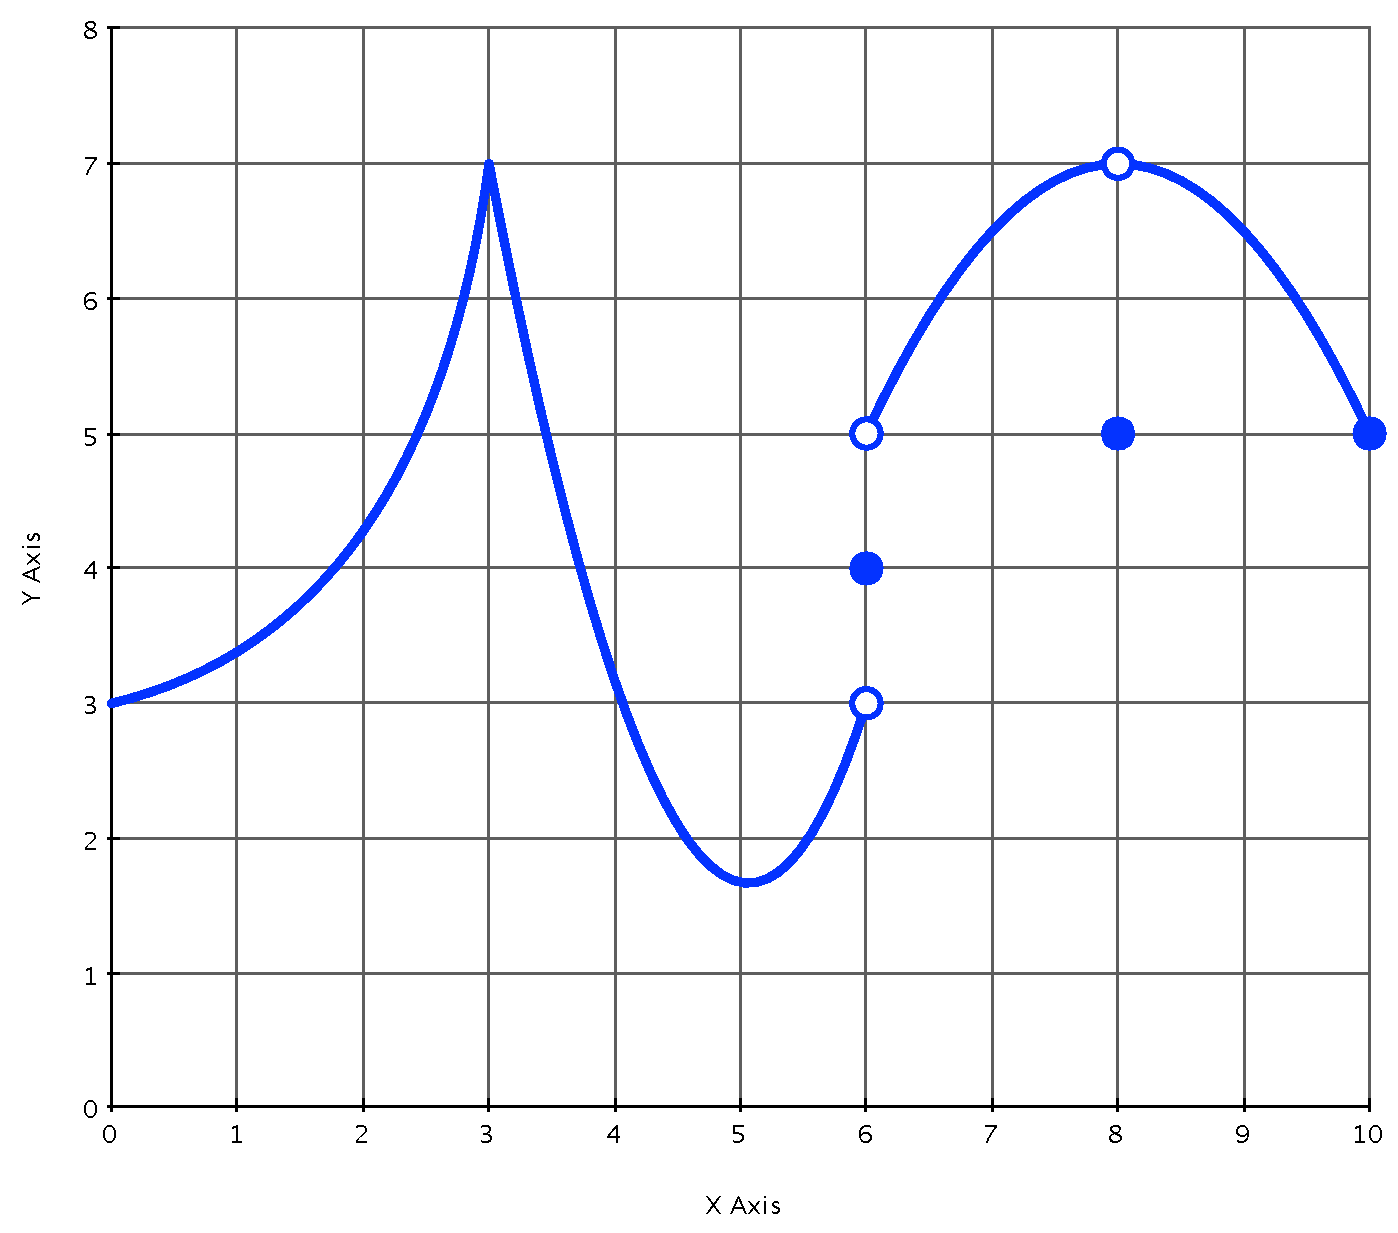
\includegraphics[width=0.5\textwidth]{a1-plot2}
\end{center}
State the value of each of the following. If a value does not exist, write ``DNE''. You do NOT need to explain your answers on this problem; only the answer will be graded. 

\begin{parts}
	\part[2] $g'(5)$ 
	\vspace{0.5in}
	
	\part[2] $\displaystyle{\lim_{x \to 8} g(x)}$ 
	\vspace{0.5in}
	
	\part[2] $\displaystyle{\lim_{x \to 6^+} g(x)}$
	\vspace{0.5in}
	
	\part[3] The points on the interval $(0,10)$ at which $f$ fails to be continuous
	\vspace{1in}
	
	
	
	\part[3] The points on the interval $(0,10)$ at which $f$ fails to be differentiable  
	\vspace{1in}
	
\end{parts}

\pageturn 

\question An object is moving in such a way that its position $s$ (in meters) at time $t$ (in seconds) by the function $s(t) = 8t^2 - 10t + 100$. 
	\begin{parts}
		\part[12] Use the limit definition of the derivative to find a formula for $s'(t)$. You must use the limit definition and show all your work, both algebra and limit-taking, to receive credit for this problem. 
		
		\vspace{4in}
		
		\part[4] Find the object's instantaneous velocity at $t = 1$. Show your work and state the units of your answer. 
		
	\end{parts}

\pageturn

\question The population of a small town is given by $P(t) = 2000(1.02)^t$ where $P$ is in people and $t$ is in years since 1980. 
	\begin{parts}
		\part[8] Set up -- \emph{but do not evaluate} -- an expression involving limits that would find the instantaneous rate of change in the town's population in the year 2013. 
		
		\vspace{1in}
		
		\part[4] Suppose we wanted to evaluate the above limit expression using only algebraic operations and no numerical or graphical estimation. Do you think this method of solution would be appropriate for this problem? Explain. 
				
		\vspace{1.7in}
		
		
		\part[8] Here is a graph of $P(t)$ along with the tangent line to the graph of $P$ when $t = 25$. Use these to estimate the instantaneous rate of change in the population of the town in 2005. State your answer clearly and  explain in one sentence how you got your answer. 
		
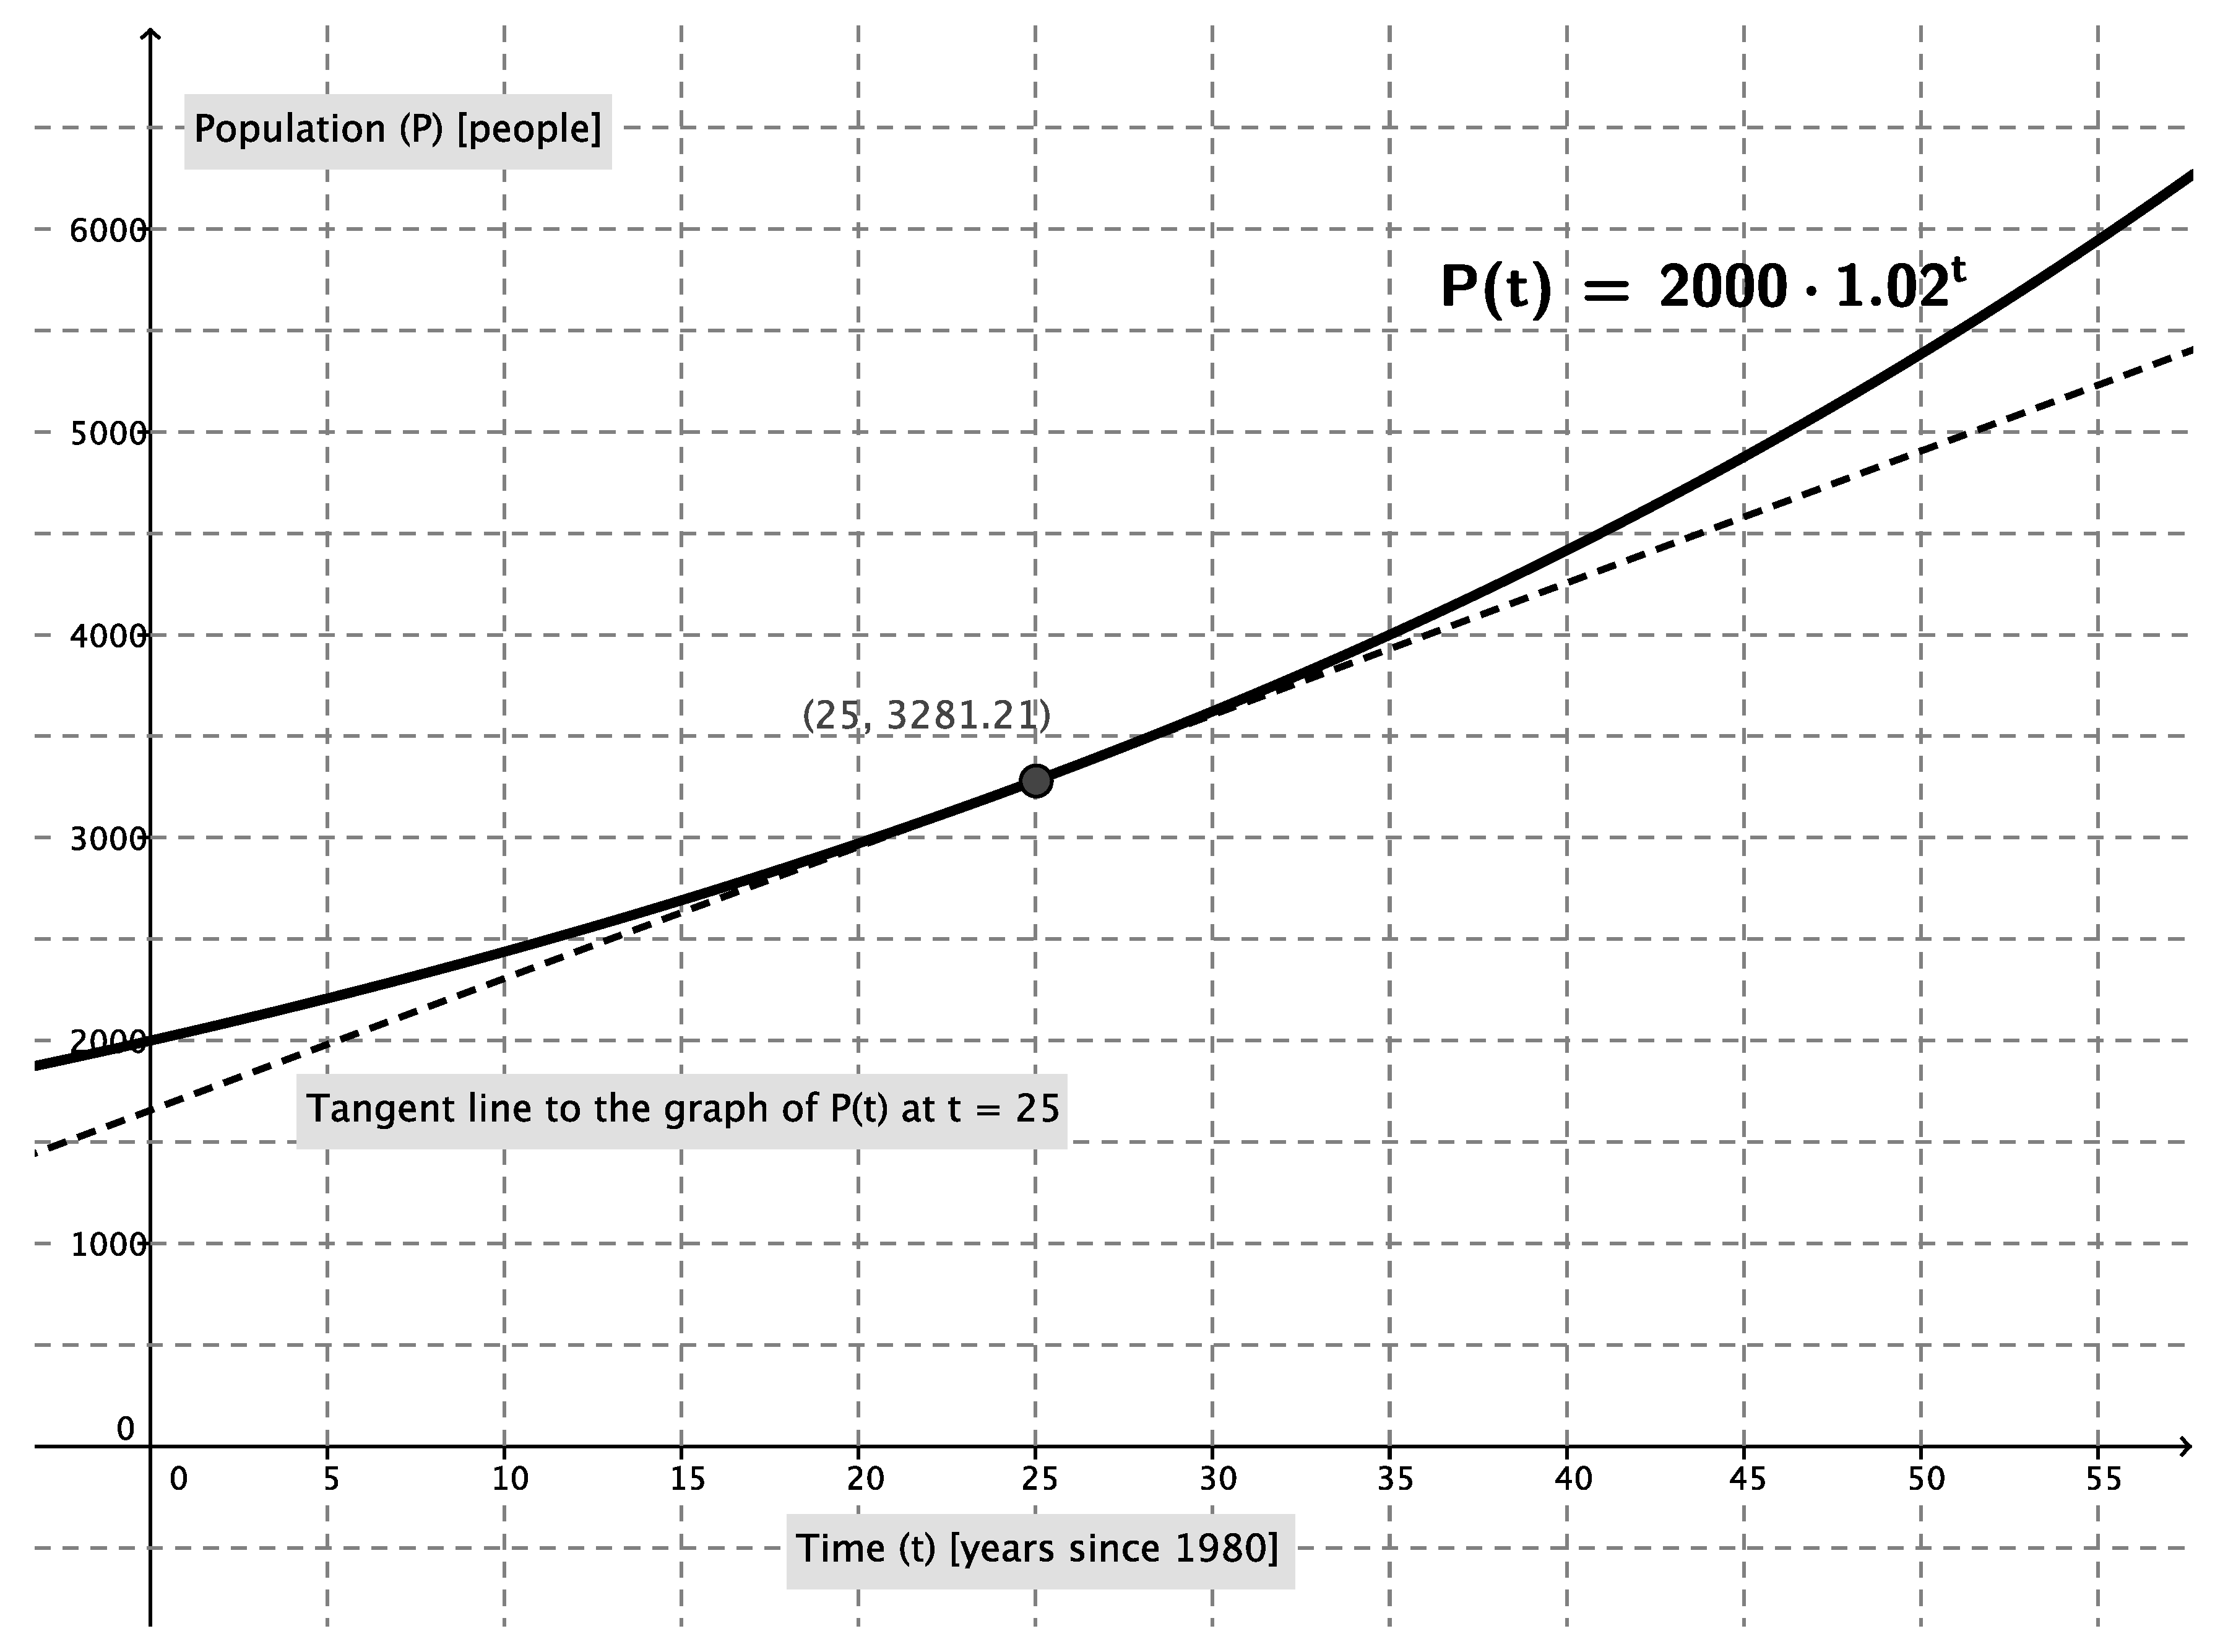
\includegraphics[width=0.6\textwidth]{a1-plot3}
		
		\vspace{0.5in}
		
		\part[4] Suppose a student did part (c) of this problem and came up with an answer of $-450$. Is  this solution reasonable and consistent with practical considerations? Explain your reasoning. 
		
		
		
	\end{parts}



% \question Below is the graph of a function $y = f(x)$, with four points ($A,B,C,D$) marked on it. 
% \begin{center}
% 	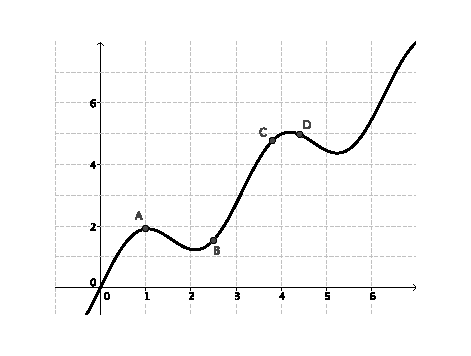
\includegraphics[width=0.5\textwidth]{a1-plot1}
% \end{center}
% Using this graph, answer the following questions. 
% 	\begin{parts}
% 		\part[4] What is (approximately) the value of the derivative $f'(x)$ at the point $A$? State your answer clearly and explain your reasoning in one sentence. 
% 		
% 		\vspace{1.5in}
% 		
% 		\part[4] Is the value of the second derivative $f''(x)$ positive, negative, or zero at point $A$? State your answer clearly and explain your reasoning in one sentence. 
% 		
% 		\vspace{1.5in}
% 		
% 		\part[4] Which is greater: The value of the derivative $f'(x)$ at point $B$, or the value of the derivative at point $C$? State your answer clearly and explain your reasoning in one sentence.
% 		
% 		\vspace{1.5in}
% 		
% 		\part[4] Which is greater: The value of the second derivative $f''(x)$ at point $B$, or the value of the second derivative $f''(x)$ at point $D$?  State your answer clearly and explain your reasoning in one sentence.  
% 		
% 	\end{parts}

\pageturn

\question The financial value of a mutual fund goes up and down over time. Suppose that a certain mutual fund's value $V$ (in dollars) is a function of time $t$ (in months since January 2010). In particular note that January 2012 corresponds to the time value $t = 24$, July 2012 is $t=30$, and January 2013 is $t = 36$. Suppose we also know the following information about the value of the mutual fund: 
\[ V(24) = 8500 \qquad V(30) = 8700 \qquad V(36) = 10300 \qquad V'(36) = 200 \qquad V''(36) = -30 \] 
	\begin{parts}
		\part[6] Find the average rate of change in the value of the mutual fund from January 2012 to July 2012. Show your work and put correct units on your answer. 
		
		\vspace{1.5in}
		
		\part[6] Use a central difference to approximate the value of the instantaneous rate of change in the value of the mutual fund in July 2012. Show your work and put correct units on your answer. 
		
		\vspace{1.5in}
		
		
		\part[6] Find the local linearization of $V$ when $t=36$, and then use the local linearization to predict the value of the mutual fund in July 2013. 
		
		
		\vspace{2in}
		
		\part[4] Which is more likely to be greater: The actual value of the mutual fund in July 2013, or the estimated value you calculated in part (c)? Explain your reasoning, and base your reasoning only on the data presented in this problem. 
	\end{parts}

\pageturn

\question[6] Your response to the last question on this Assessment is to be typed up in an email and submitted to me (talbertr@gvsu.edu) no later than 5pm on Saturday, September 21. In this question, I am just soliciting your honest feedback on how the course is going so far. Please include anything you feel would be helpful in improving the course moving forward. You won't be penalized if you don't like everything (or anything!) and I certainly value your constructive criticism. The questions to address are: 
\begin{itemize}
	\item What's been your favorite thing about the course so far? 
	\item What's one thing you would like to see changed (that can be changed) and how would you change it? 
	\item In particular, how has the ``flipped'' setup of the course (lectures done outside of class; class time spent on activity) worked for you so far? 
	\item Anything else you want to mention? 
\end{itemize}

\end{questions}


\end{document}